\documentclass[fleqn, 11pt]{article}
\usepackage{float}
\usepackage{graphicx}
\usepackage{caption}
\usepackage{subcaption}
\usepackage{enumitem}
\usepackage{booktabs}
\usepackage[portuges]{babel}
\usepackage[utf8x]{inputenc}
\usepackage{comment}
\usepackage{fullpage}
\usepackage{xcolor}
\usepackage{amsmath,amsfonts,amssymb,amsthm, bm}
\usepackage{csvsimple}

\usepackage{listings}
\usepackage{color}
\usepackage{tikz}
\usetikzlibrary{positioning,decorations.pathreplacing}
\usepackage{hyperref}


\definecolor{mygreen}{RGB}{28,172,0}
\definecolor{mylilas}{RGB}{170,55,241}
\renewcommand{\min}{\expandafter\,\operatorname*{min}}

% Default fixed font does not support bold face
\DeclareFixedFont{\ttb}{T1}{txtt}{bx}{n}{12} % for bold
\DeclareFixedFont{\ttm}{T1}{txtt}{m}{n}{12}  % for normal

% Custom colors
\usepackage{color}
\definecolor{deepblue}{rgb}{0,0,0.5}
\definecolor{deepred}{rgb}{0.6,0,0}
\definecolor{deepgreen}{rgb}{0,0.5,0}

\usepackage{listings}

% Python style for highlighting
\newcommand\pythonstyle{\lstset{
language=Python,
basicstyle=\ttm,
otherkeywords={self},             % Add keywords here
keywordstyle=\ttb\color{deepblue},
emph={MyClass,__init__},          % Custom highlighting
emphstyle=\ttb\color{deepred},    % Custom highlighting style
stringstyle=\color{deepgreen},
frame=tb,                         % Any extra options here
showstringspaces=false            % 
}}


% Python environment
\lstnewenvironment{python}[1][]
{
\pythonstyle
\lstset{#1}
}
{}

% Python for external files
\newcommand\pythonexternal[2][]{{
\pythonstyle
\lstinputlisting[#1]{#2}}}

% Python for inline
\newcommand\pythoninline[1]{{\pythonstyle\lstinline!#1!}}


\begin{document}
\noindent
\large\textbf{Lista de Exercícios 2} \hfill \textbf{Luis Vinicius Costa Silva} \\
\normalsize Otimização Clássica \\
Prof. Romes Antonio Borges \\
\hfill Data de Entrega: 27/05/2019

\section*{Questão 1}
Os seguintes métodos de otimização foram implementados:

\begin{itemize}
\item[•] Ordem Zero:
   \subitem \hyperref[buscaAleatoria]{Busca Aleatória}
   \subitem \hyperref[secaoAurea]{Seção Áurea}
   \subitem \hyperref[fibonacci]{Fibonacci}
   \subitem \hyperref[nelderMead]{Polítopo}
   \subitem \hyperref[powell]{Powell}
      
\item[•] Ordem Um:
   \subitem \hyperref[maximaDescida]{Máxima Descida}
   \subitem \hyperref[gradienteConjugado]{Gradiente Conjugado}
   
\item[•] Ordem Dois:
   \subitem \hyperref[newton]{Newton}
   
\item[•] Quasi-Newton:   
   \subitem \hyperref[bfgs]{BFGS-DFP}

\item[•] Outros:
   \subitem \hyperref[interpol]{Interpolação Polinomial}   
\end{itemize}

Métodos de Ordem Zero tem como entrada apenas um intervalo de busca, um chute inicial (opcional em alguns casos) e a própria função a ser otimizada. Estes algoritmos utilizam apenas o valor de um determinado $X$ na função a fim de computar o ponto ótimo.\newline

Métodos de Primeira Ordem acrescentam a primeira derivada (ou gradiente no caso de otimização multivariável) a entrada do algoritmo, enquanto que Métodos de Segunda Ordem utilizam-se da segunda derivada (ou hessiana no caso de otimização multivariável). \newline

A derivada de primeira ordem sinaliza o decréscimo ou incremento da função em um determinado ponto, ou seja a derivada primeira ordem serve como uma linha tangente a um ponto em sua superfície de erro. Nos métodos de segunda ordem, a informação da derivada segunda denota o incremento/decremento da primeira derivada, indicando as características da curvatura da função (e.g: côncava/convexa).\newline

Métodos Quasi-Newton são similares aos Métodos de Segunda Ordem, com a diferença de que ao invés de usarem a hessiana da função na regra de atualização, esta é substituída por um termo aproximado, que converge (em situações ideais) para a hessiana exata, geralmente estes métodos são classificados como Métodos de Ordem Zero ou à parte.\newline

O método de Interpolação Polinomial não tem como propósito minimizar uma função diretamente, ao invés disso, este método computa um polinômio que tem como pontos pré-determinados uma entrada do usuário. Tal algoritmo se faz útil em problemas de minimização através da simplificação da função original (ou um intervalo em particular da mesma) em um polinômio, e a busca subsequente do mínimo da mesma através da aplicação de um método de otimização no polinômio computado anteriormente. Neste trabalho, o algoritmo de interpolação polinomial implementado consiste na montagem da matriz de Vandermonde e a aplicação da eliminação da eliminação Gaussiana a fim de obter os coeficientes $\alpha$ do polinômio contidos na dita matriz.

\section*{Questão 2}
Dada as funções abaixo, foram computados seus respectivos mínimos através do Método de Fibonacci e Método da Seção Áurea:
\begin{enumerate}[label=(\alph*)]
\item \hyperref[Q2A]{$F(x_1) = 3 x_1^2-5 x_1$ \hfill $0.0 \leq x_1 \leq 3.0$}
\item \hyperref[Q2B]{$F(x_1) = (x_1-3)^2    $ \hfill $0.0 \leq x_1 \leq 10$}
\item \hyperref[Q2C]{$F(x_1) = \frac{(\sin(0.1+2 x_1))}{(1+x_1)}$ \hfill $0.5 \leq x_1 \leq 3.5$  }
\end{enumerate}

Sabe-se que os mínimos são respectivamente:
\begin{enumerate}[label=(\alph*)]
\item $x_1 = \frac{5}{6}$
\item $x_1 = 3$
\item $x_1 \approx 2.22939$
\end{enumerate}

%slides 25 e 47

As duas primeiras iterações do método da Seção Áurea são realizadas da seguinte forma:
\newline

\hfill Iteração 1 do método da Seção Áurea na Função (a):
\begin{align*}
\begin{split}
\hfill \alpha_1 = a_1 + \rho (b_1-a_1) \approx 0 + 0.3820 (3-0) = 1.597 \\
\hfill \beta_1 = a_1 + (1 - \rho) (b_1 - a_1) \approx 0 + 0.6180 (3 - 0) = 2.584 \\
\hfill f(\alpha_1) \approx 0.0 \\ 
\hfill f(\beta_1) \approx   7.1111  \\
\hfill f(\beta_1) \geq f(\alpha_1) \\
\hfill x^* \in [a, \beta_1] = [0, 2.584]
\end{split}
\end{align*}
\newline

\hfill Iteração 2 do método da Seção Áurea na Função (a):
\begin{align*}
\begin{split}
\hfill \alpha_2 = a_2 + \rho (b_2-a_2) \approx 0 + 0.3820 (7.1111-0) = 0.987 \\
\hfill \beta_2 = a_2 + (1 - \rho) (b_2 - a_2) \approx 0 + 0.6180 (7.1111 - 0) = 1.597 \\
\hfill f(\alpha_2) \approx -0.3337 \\ 
\hfill f(\beta_2) \approx   7.1111  \\
\hfill f(\beta_2) \geq f(\alpha_2) \\
\hfill x^* \in [a, \beta_2] = [0, 1.597]
\end{split}
\end{align*}
\newline

\hfill Iteração 1 do método Fibonacci na Função (a):
\begin{align*}
\begin{split}
\hfill n = 18 \\
\hfill F_18/F_17 \approx 0.382 \\
\hfill \alpha_1 = a_1 + \rho_1 (b_1 - a_1) \approx 1.597 \\
\hfill \beta_1 = a_1 + (1 - \rho_1) (b_1 - a_1) \approx 2.584 \\
\hfill f(\alpha_1) \approx 0.0 \\
\hfill f(\beta_1) \approx 7.111 \\
\hfill f(\beta_1) \geq f(\alpha_1) \\
\hfill x* \in [a, \beta_1] = [0. 2.584]
\end{split}
\end{align*}

\hfill Iteração 2 do método Fibonacci na Função (a):
\begin{align*}
\begin{split}
\hfill \alpha_2 = a_2 + \rho_2 (b_2 - a_2) \approx 0.987 \\
\hfill \beta_2 = a_2 + (1 - \rho_2) (b_2 - a_2) \approx 1.597 \\
\hfill f(\alpha_2) \approx -0.3337 \\
\hfill f(\beta_2) \approx 7.1111 \\
\hfill f(\beta_2) \geq f(\alpha_1) \\
\hfill x* \in [a, \beta_2] = [0. 1.597]
\end{split}
\end{align*}


As figuras abaixo representam o gráfico das funções e o mínimo computado por cada algoritmo, assim como detalhes da convergência dos mesmos:

\begin{figure}[H]
\centering
\begin{subfigure}{.5\textwidth}
  \centering
  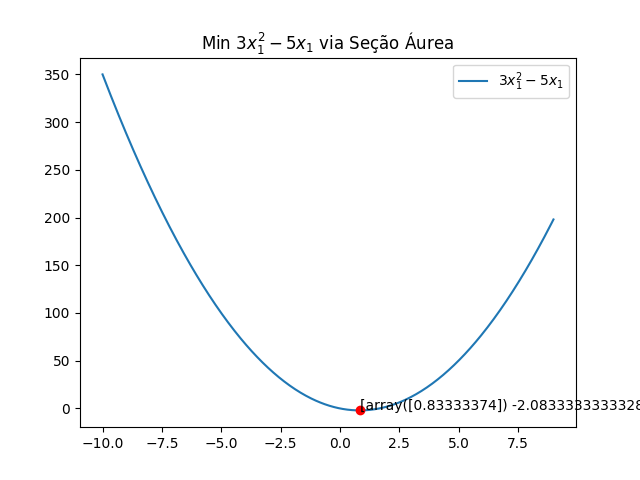
\includegraphics[width=\linewidth]{Q2/aSA.png}
  %\caption{A subfigure}
\end{subfigure}%
\begin{subfigure}{.5\textwidth}
  \centering
  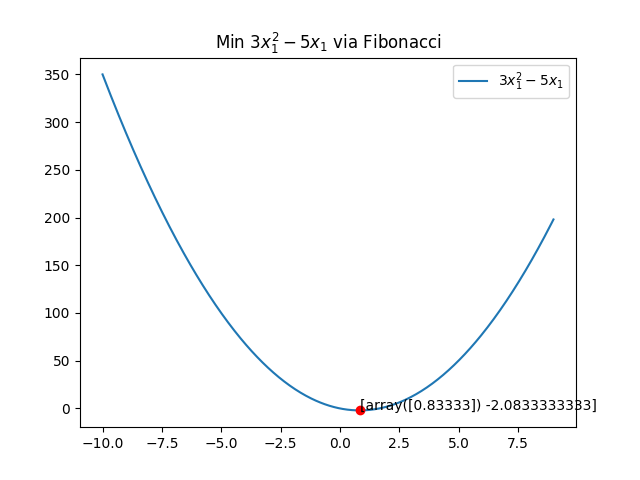
\includegraphics[width=\linewidth]{Q2/aFib.png}
  %\caption{A subfigure}
\end{subfigure}

\centering
\begin{subfigure}{.5\textwidth}
  \centering
  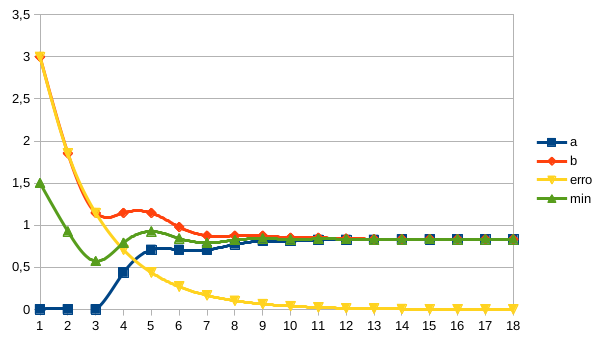
\includegraphics[width=\linewidth]{Q2/aSAConv.png}
  \caption{Seção Áurea}
\end{subfigure}%
\begin{subfigure}{.5\textwidth}
  \centering
  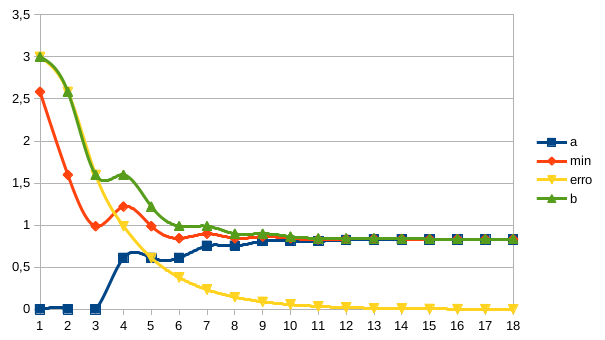
\includegraphics[width=\linewidth]{Q2/aFibConv.png}
  \caption{Fibonacci}
\end{subfigure}
\caption{Questão 2 -- Letra A - Mínimos Computados e \\ convergência dos algoritmos}
\label{Q2A}
\end{figure}


\begin{figure}[H]
\centering
\begin{subfigure}{.5\textwidth}
  \centering
  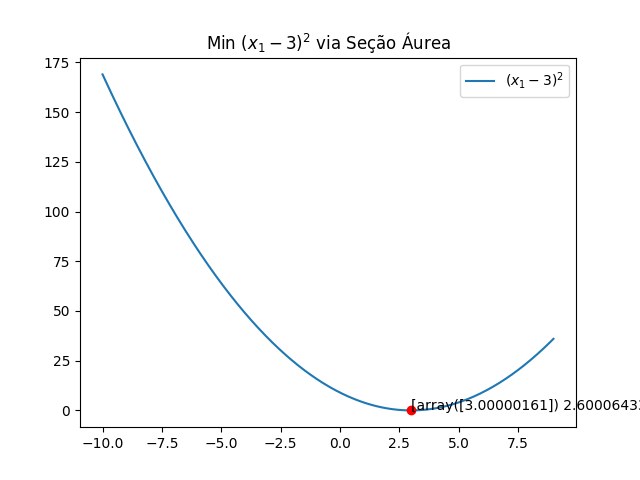
\includegraphics[width=\linewidth]{Q2/bSA.png}
  %\caption{A subfigure}
\end{subfigure}%
\begin{subfigure}{.5\textwidth}
  \centering
  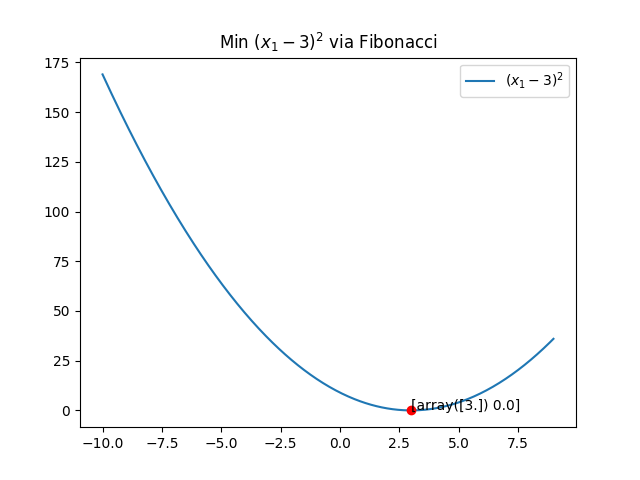
\includegraphics[width=\linewidth]{Q2/bFib.png}
  %\caption{A subfigure}
\end{subfigure}

\centering
\begin{subfigure}{.5\textwidth}
  \centering
  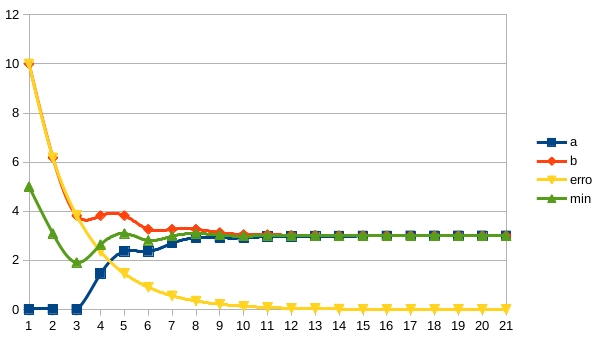
\includegraphics[width=\linewidth]{Q2/bSAConv.png}
  \caption{Seção Áurea}
\end{subfigure}%
\begin{subfigure}{.5\textwidth}
  \centering
  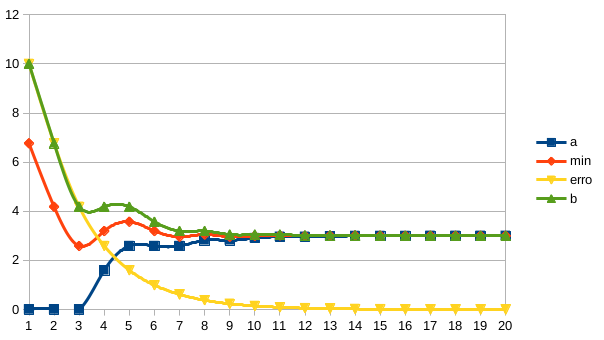
\includegraphics[width=\linewidth]{Q2/bFibConv.png}
  \caption{Fibonacci}
\end{subfigure}
\caption{Questão 2 -- Letra B - Mínimos Computados e \\ convergência dos algoritmos}
\label{Q2B}
\end{figure}

\begin{figure}[H]
\centering
\begin{subfigure}{.5\textwidth}
  \centering
  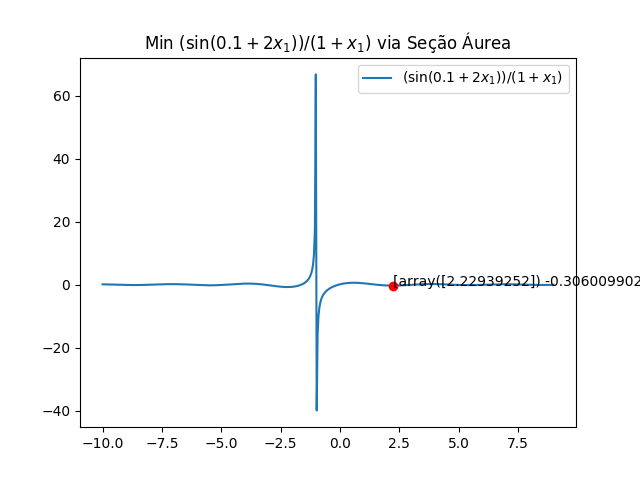
\includegraphics[width=\linewidth]{Q2/cSA.png}
  %\caption{A subfigure}
\end{subfigure}%
\begin{subfigure}{.5\textwidth}
  \centering
  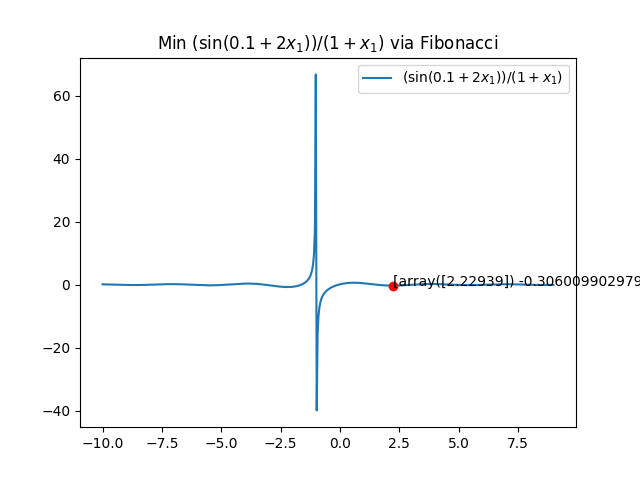
\includegraphics[width=\linewidth]{Q2/cFib.png}
  %\caption{A subfigure}
\end{subfigure}

\centering
\begin{subfigure}{.5\textwidth}
  \centering
  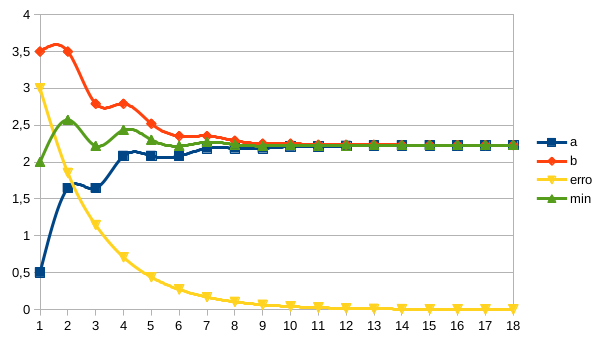
\includegraphics[width=\linewidth]{Q2/cSAConv.png}
  \caption{Seção Áurea}
\end{subfigure}%
\begin{subfigure}{.5\textwidth}
  \centering
  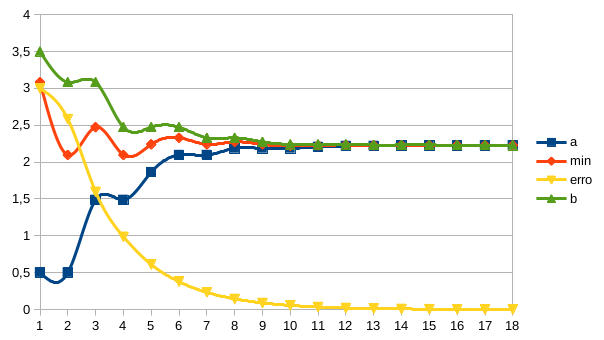
\includegraphics[width=\linewidth]{Q2/cFibConv.png}
  \caption{Fibonacci}
\end{subfigure}
\caption{Questão 2 -- Letra C - Mínimos Computados e \\ convergência dos algoritmos}
\end{figure}

\begin{figure}[H]
\centering
\begin{subfigure}{.5\textwidth}
  \centering
  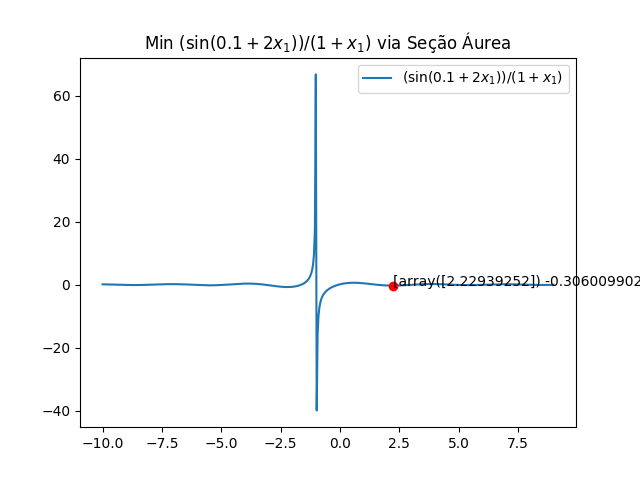
\includegraphics[width=\linewidth]{Q2/cSA.png}
  %\caption{A subfigure}
\end{subfigure}%
\begin{subfigure}{.5\textwidth}
  \centering
  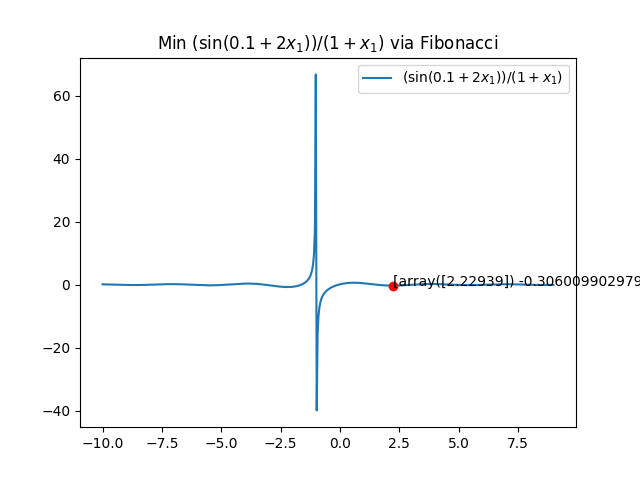
\includegraphics[width=\linewidth]{Q2/cFib.png}
  %\caption{A subfigure}
\end{subfigure}

\centering
\begin{subfigure}{.5\textwidth}
  \centering
  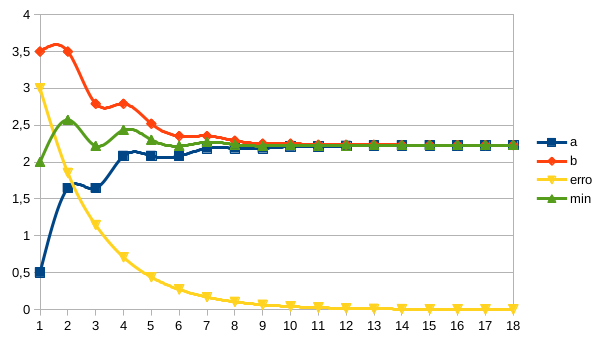
\includegraphics[width=\linewidth]{Q2/cSAConvInterpol.png}
  \caption{Seção Áurea}
\end{subfigure}%
\begin{subfigure}{.5\textwidth}
  \centering
  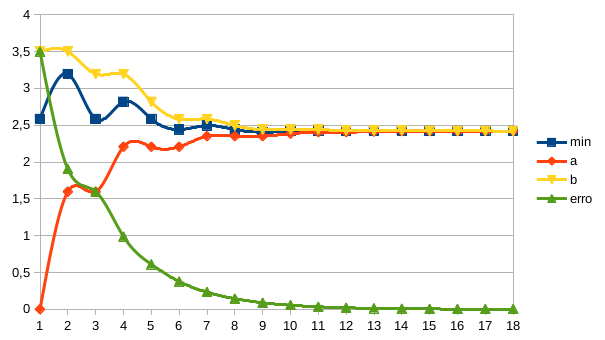
\includegraphics[width=\linewidth]{Q2/cFibConvInterpol.png}
  \caption{Fibonacci}
\end{subfigure}
\label{Q2C}
\caption{Questão 2 -- Letra C -- Versão Interpolada \\ Mínimos Computados e convergência dos algoritmos}
\end{figure}

Os gráficos de convergência foram gerados a partir dos arquivos CSV anexos a este relatório. Os algoritmos foram executados com as funções listadas acima sob tolerância de $10^{-3}$. Nota-se que ambos os 
algoritmos obtiveram o $x*$ na mesma quantidade de iterações em todos os casos (com exceção da \hyperref[Q2B]{letra 
B} com 1 iteração de diferença), algo esperado visto que ambos possuem uma razão de convergência similar. Além disso, 
nota-se que os intervalos delimitados por $a$ e $b$ foram reduzidos de maneira similar nas diversas execuções, visto 
que a sequência de tais termos sobre as iterações possuem r-convergência linear com coeficiente $\tau \approx 0.618$. 
É possível concluir tal fato através das análises experimentais do algoritmo, e de forma contundente, pelo fato de 
que a cada iteração, o tamanho do intervalo contendo o mínimo de $f(x)$ é reducido por $\tau$, de tal forma que $b_k 
- a_k = \tau^k (b_0 - a_0)$. Visto que $x* \in [a_k,b_k] \forall k \in \mathbb{N}$, temos que:

\begin{equation}
\begin{split}
(b_k-x*) \leq (b_k-a_k) \leq \tau^k (b_0-a_0) \\
(x-a_k) \leq (b_k-a_k) \leq \tau^k (b_0-a_0)
\end{split}
\end{equation}

Foram gerados três polinômios interpoladores com $N$ pontos equidistantes, onde $N$ foi a diferença entre os intervalos $a$ e $b$ de interesse de cada função respectivamente. Logo, foram gerados os polinômios com os pontos abaixo:

\begin{table}[H]
\centering
\begin{tabular}{lll|l|l|lll}
\cline{1-2} \cline{4-5} \cline{7-8}
\multicolumn{2}{|l|}{Letra A} &  & \multicolumn{2}{l|}{Letra B} & \multicolumn{1}{l|}{} & \multicolumn{2}{l|}{Letra C} \\ \cline{1-2} \cline{4-5} \cline{7-8} 
\multicolumn{1}{|l|}{x} & \multicolumn{1}{l|}{f(x)} &  & x & f(x) & \multicolumn{1}{l|}{} & \multicolumn{1}{l|}{x} & \multicolumn{1}{l|}{f(x)} \\ \cline{1-2} \cline{4-5} \cline{7-8} 
\multicolumn{1}{|l|}{0} & \multicolumn{1}{l|}{0} &  & 0 & 9 & \multicolumn{1}{l|}{} & \multicolumn{1}{l|}{0} & \multicolumn{1}{l|}{0,09983341664682815} \\ \cline{1-2} \cline{4-5} \cline{7-8} 
\multicolumn{1}{|l|}{1} & \multicolumn{1}{l|}{-2} &  & 1 & 4 & \multicolumn{1}{l|}{} & \multicolumn{1}{l|}{1} & \multicolumn{1}{l|}{0,43160468332443686} \\ \cline{1-2} \cline{4-5} \cline{7-8} 
\multicolumn{1}{|l|}{2} & \multicolumn{1}{l|}{2} &  & 2 & 1 & \multicolumn{1}{l|}{} & \multicolumn{1}{l|}{2} & \multicolumn{1}{l|}{-0,2727590370214701} \\ \cline{1-2} \cline{4-5} \cline{7-8} 
\multicolumn{1}{|l|}{3} & \multicolumn{1}{l|}{12} &  & 3 & 0 & \multicolumn{1}{l|}{} & \multicolumn{1}{l|}{3} & \multicolumn{1}{l|}{-0,04554062606802397} \\ \cline{1-2} \cline{4-5} \cline{7-8} 
 &  &  & 4 & 1 &  &  &  \\ \cline{4-5}
 &  &  & 5 & 4 &  &  &  \\ \cline{4-5}
 &  &  & 6 & 9 &  &  &  \\ \cline{4-5}
 &  &  & 7 & 16 &  &  &  \\ \cline{4-5}
 &  &  & 8 & 25 &  &  &  \\ \cline{4-5}
 &  &  & 9 & 36 &  &  &  \\ \cline{4-5}
\end{tabular}
\caption{Pontos gerados para criação do polinômio interpolador}
\label{Q2Pontos}
\end{table}
Os pontos gerados para os itens (a) e (b) resultaram na função original do exercício, logo os $x's*$ encontrandos foram os mesmos, esta "coincidência" resulta do fato de que a interpolação de pontos equidistantes de um polinômio gera o próprio polinômio (ver algoritmo de Gregory-Newton). Visto que o item (c) não era um polinômio, a função interpolada não foi exatamente igual a função original, o polinômio obtido $0.327952853053811 x^3 - 1.50192605267319 x^2 + 1.50574446629699 x + 0.0998334166468282$ teve como mínimo no intervalo $[0.5, 3.5] \in \mathbb{R}$ um $x* = 2.420$ e $x*=2.421$, obtidos respectivamente com o algoritmo da Seção Áurea e Fibonacci, uma aproximação aceitável do $x*$ encontrado para a solução exata, sendo este igual a $2.229$. Alternativamente foi obtida a derivada do polinômio interpolador, e igualando-o a zero, obtendo-se as raízes da parábola como $x_1 = 0.63216286445301$ e $x_2 = 2.4209712241569$, sendo $x_2$ o mínimo do polinômio interpolador novamente. Embora ambos os algoritmos gastaram a mesma quantidade de iterações para minimizar a função original e a interpolada, é sabido que a interpolação de um intervalo da função e a posterior computação do mínimo sob a função interpolada tende a ser menos custoso computacionalmente em alguns casos (onde a avaliação da função original é computacionalmente cara) ao custo de uma considerável perda de precisão na computação do $x*$ da função real (visto que a interpolação pode não representar fielmente a função original).
\newpage

\section*{Questão 3}
Dada as funções abaixo, foram computados seus respectivos mínimos através dos métodos numéricos listados na \hyperref[Q1]{Questão 1}, para cada execução foi analisada a convergência do método. 
\begin{enumerate}[label=(\alph*)]
\item \hyperref[Q3A]{$F(x_1) = "x_1^2 - 3 x_1 x_2 + 4 x_2^2 + x_1 - x_2"$}
\item \hyperref[Q3B]{$F(x_1) = 6 x_1^2 + 2 x_2^2 - 6 x_1 x_2 - x_1 - 2 x_2$}
\item \hyperref[Q3B]{$F(x_1) = x_1 - x_2 + 2 x_1^2 + 2 x_1 x_2 + x_2^2$  }
\end{enumerate}

É sabido que os mínimos de tais funções são respectivamente $\big (-\frac{5}{7},-\frac{1}{7} \big )$, $\big ( \frac{4}{3},\frac{5}{2} \big )$ e $\big  (-1,\frac{3}{2} \big )$.

Abaixo pode-se observar os gráficos dos mínimos computados de cada função e a convergência de cada algoritmo: 

\begin{figure}[H]
\center{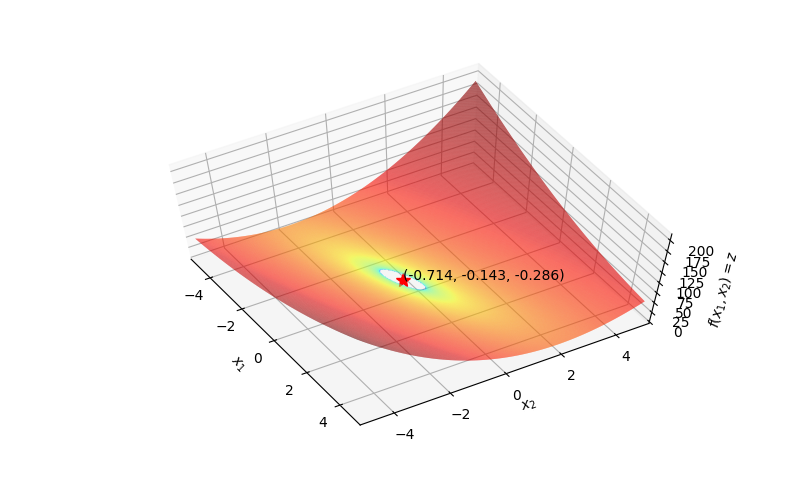
\includegraphics[width=0.5\textwidth]
	{Q3/1.png}}
  \caption{$\min f(X) = x_1^2 - 3 x_1 x_2 + 4 x_2^2 + x_1 - x_2$}
\end{figure}


\begin{figure}[H]
\center{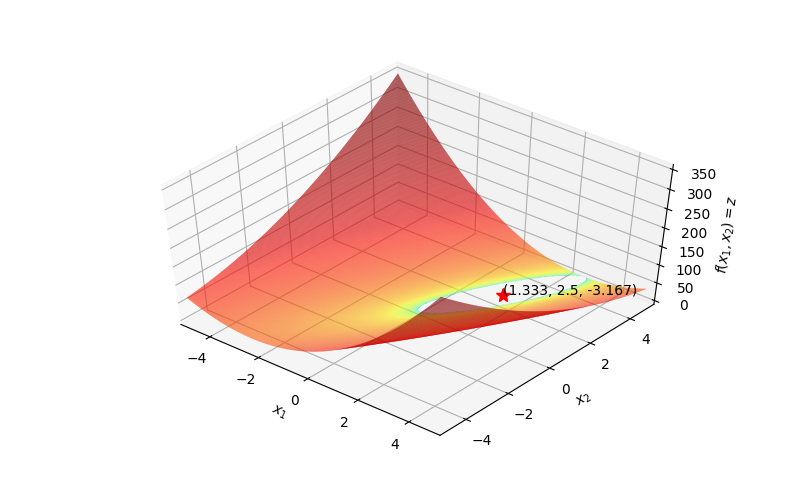
\includegraphics[width=0.5\textwidth]
	{Q3/2.png}}
  \caption{$\min f(X) = 6 x_1^2 + 2 x_2^2 - 6 x_1 x_2 - x_1 - 2 x_2$}
\end{figure}


\begin{figure}[H]
\center{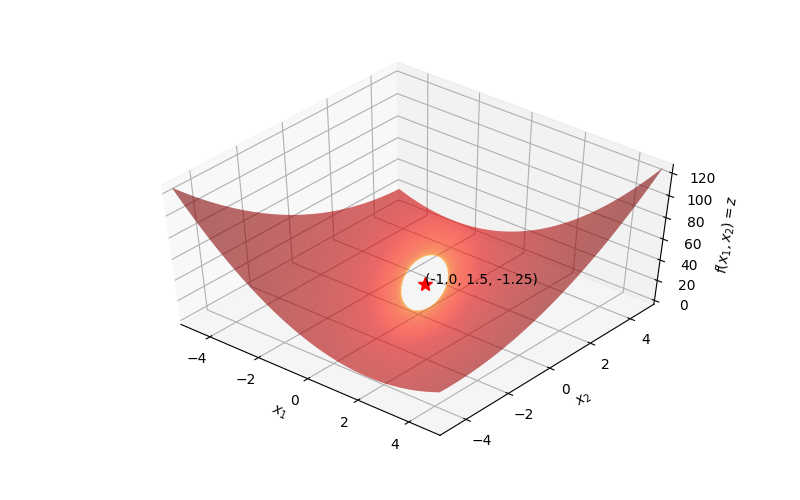
\includegraphics[width=0.5\textwidth]
	{Q3/3.png}}
  \caption{$\min f(X) = x_1^2 - 3 x_1 x_2 + 4 x_2^2 + x_1 - x_2$}
\end{figure}


\begin{figure}[H]
\centering
\begin{subfigure}{.5\textwidth}
  \centering
  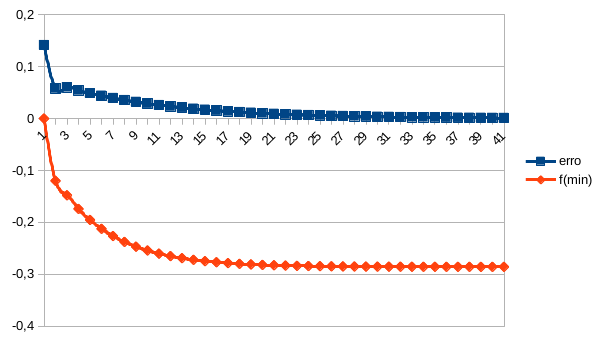
\includegraphics[width=\linewidth]{Q3/A_BFGS.png}
  %\caption{A subfigure}
\end{subfigure}%
\begin{subfigure}{.5\textwidth}
  \centering
  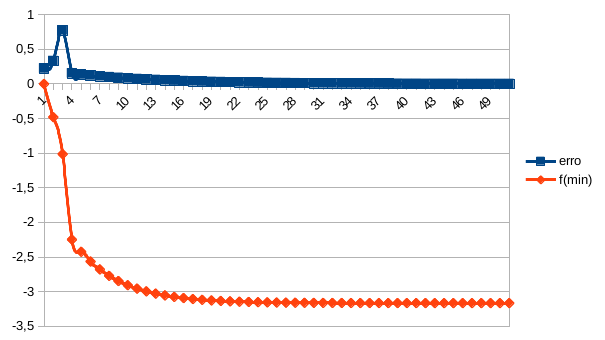
\includegraphics[width=\linewidth]{Q3/B_BFGS.png}
  %\caption{A subfigure}
\end{subfigure}
\begin{subfigure}{.5\textwidth}
  \centering
  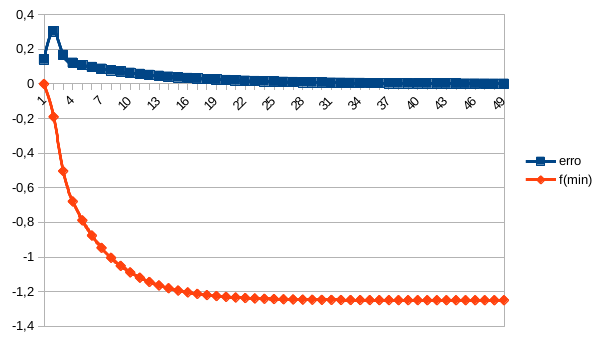
\includegraphics[width=\linewidth]{Q3/C_BFGS.png}
  %\caption{A subfigure}
\end{subfigure}
\caption{Método BFGS sendo executado com as funções (a), (b) e (c)}
\end{figure}

\begin{figure}[H]
\centering
\begin{subfigure}{.5\textwidth}
  \centering
  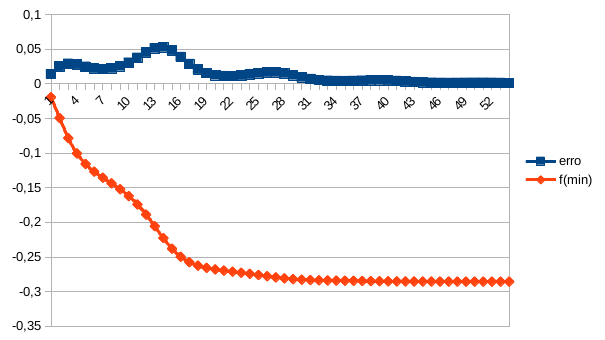
\includegraphics[width=\linewidth]{Q3/A_GradConjugado.png}
  %\caption{A subfigure}
\end{subfigure}%
\begin{subfigure}{.5\textwidth}
  \centering
  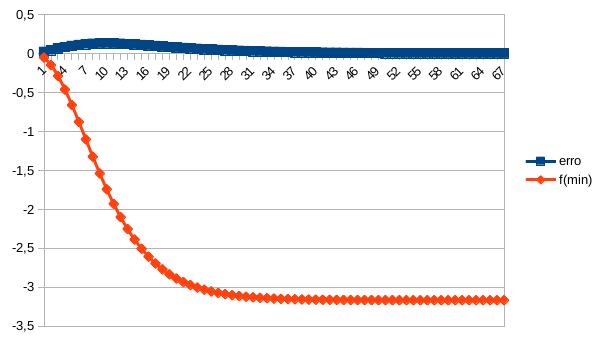
\includegraphics[width=\linewidth]{Q3/B_GradConjugado.png}
  %\caption{A subfigure}
\end{subfigure}
\begin{subfigure}{.5\textwidth}
  \centering
  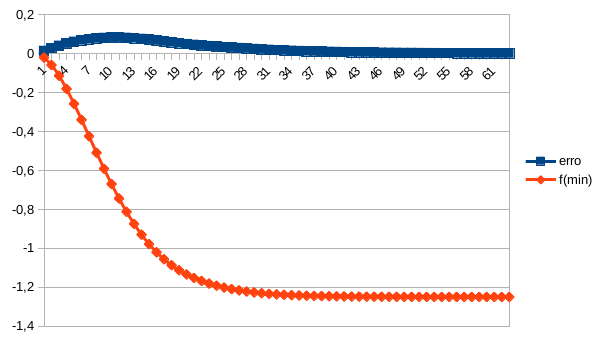
\includegraphics[width=\linewidth]{Q3/C_GradConjugado.png}
  %\caption{A subfigure}
\end{subfigure}
\caption{Método do Gradiente Conjugado sendo executado com as funções (a), (b) e (c)}
\end{figure}

\begin{figure}[H]
\centering
\begin{subfigure}{.5\textwidth}
  \centering
  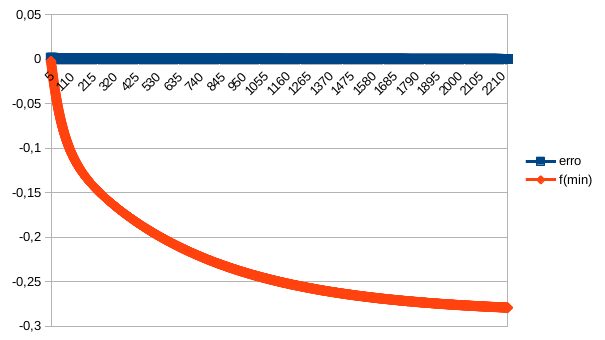
\includegraphics[width=\linewidth]{Q3/A_MaximaDescida.png}
  %\caption{A subfigure}
\end{subfigure}%
\begin{subfigure}{.5\textwidth}
  \centering
  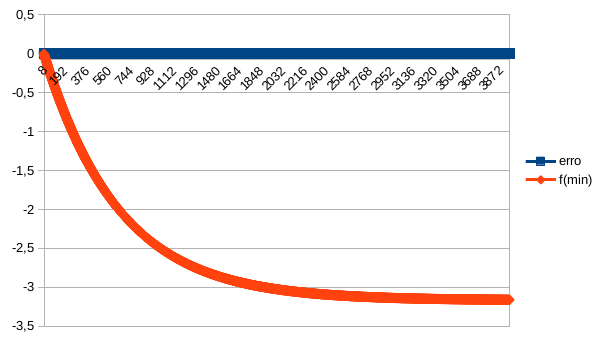
\includegraphics[width=\linewidth]{Q3/B_MaximaDescida.png}
  %\caption{A subfigure}
\end{subfigure}
\begin{subfigure}{.5\textwidth}
  \centering
  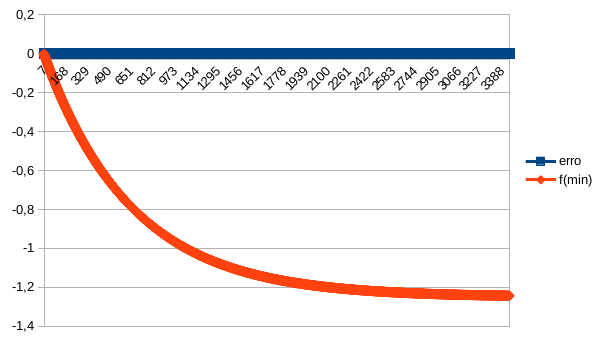
\includegraphics[width=\linewidth]{Q3/C_MaximaDescida.png}
  %\caption{A subfigure}
\end{subfigure}
\caption{Método da Máxima Descida sendo executado com as funções (a), (b) e (c)}
\end{figure}

\begin{figure}[H]
\centering
\begin{subfigure}{.5\textwidth}
  \centering
  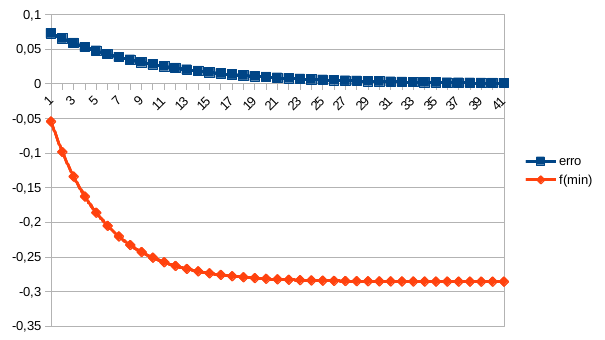
\includegraphics[width=\linewidth]{Q3/A_Newton.png}
  %\caption{A subfigure}
\end{subfigure}%
\begin{subfigure}{.5\textwidth}
  \centering
  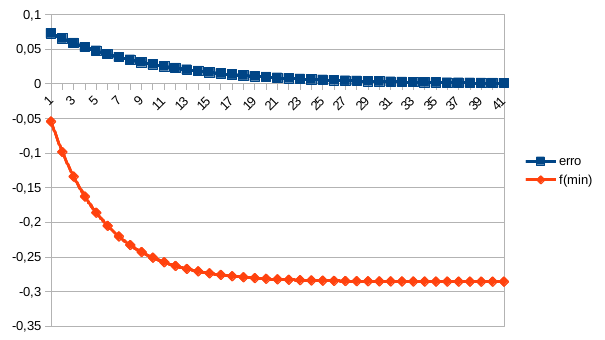
\includegraphics[width=\linewidth]{Q3/A_Newton.png}
  %\caption{A subfigure}
\end{subfigure}
\begin{subfigure}{.5\textwidth}
  \centering
  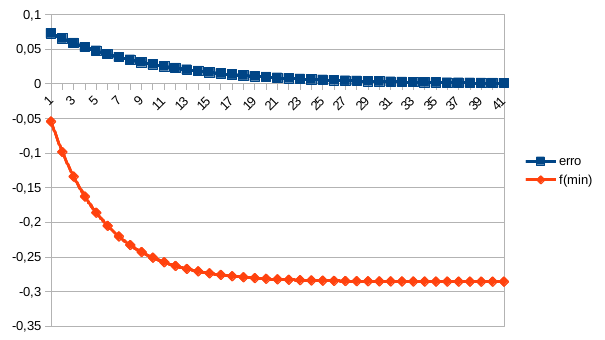
\includegraphics[width=\linewidth]{Q3/A_Newton.png}
  %\caption{A subfigure}
\end{subfigure}
\caption{Método de Newton sendo executado com as funções (a), (b) e (c)}
\end{figure}

Todos os métodos foram capazes de convergir para um $x*$ com $3$ casas decimais de precisão sob $\text{tolerância} = 10^{-5}$. Os dados utilizados para plotagem podem ser encontrados em arquivos CSV anexos a este relatório. Assim como esperava-se, métodos de segunda ordem convergem quase que imediatamente para o $x*$, visto que estes utilizam a primeira e segunda derivada da função, visto que estas foram computadas \textit{a priori}, o algoritmo implementado foi extremamente veloz, visto que não houve a necessidade de computar tais termos numericamente (é possível consultar as entradas usadas em cada método nos arquivos *.sh anexos a este relatório). Métodos Quasi-Newton como o BFGS e DFP obtiveram performance semelhante, visto que apesar de começarem com a matriz identidade como a Hessiana, esta rapidamente se torna a hessiana exata. No pior caso do BFGS, a hessiana exata foi atingida na iteração 13, enquanto que o pior caso do DFP atinge a hessiana exata na iteração 37, fazendo métodos Quasi-Newton ótimos substitutos para métodos de Segunda Ordem em aplicações de tempo real. \newline
Métodos de Ordem Um possuem um decaimento do erro da ordem de $e^{-x}$, o autor deste relatório desconhece a razão disto, mas conjectura que tal fato possa estar relacionado com o fato que algoritmos desta classe utilizam-se da informação da primeira derivada como uma linha tangente a um ponto em sua superfície de erro, e o fato de que uma série de Taylor pode ser vista como uma forma de "enumerar" todas as derivadas de $f$ em $x=b$ (isto é, se a série de Taylor de uma função é conhecida é possível extrair qualquer derivada da mesma no ponto $b$), visto que uma série de Taylor de $f$ em $x=b$ é dada por:

\begin{equation}
\sum_{n=0}^{\infty} \frac{f^{(n)}(b)}{n!} (x-b)^n
\end{equation}

Métodos de Ordem um possuem performance intermediária, computando o $x*$ em menos iterações que métodos de ordem zero, embora sejam facilmente superados por métodos de segunda ordem/Quasi-Newton neste quesito.\newline
Métodos de Ordem Zero são fáceis de implementar, mas possuem uma taxa de convergência consideravelmente lenta quando comparados a demais métodos, consequentemente estes métodos avaliam a função objetivo um número demasiado de vezes, tornando-os computacionalmente dispendiosos (e em alguns casos inviáveis). As exigências para a garantia de convergência destes métodos é a continuidade e unimodalidade da função objetivo, uma clara vantagem sobre os demais métodos visto que a diferenciabilidade da função é irrelevante para tais métodos. De forma excepcional, o algoritmo do Polítopo apresenta convergência semelhante aos métodos de Ordem Um (especialmente em modo adaptativo)\cite{gao2012implementing}.
\newpage

\section*{Códigos}
\subsection*{Método da Busca Aleatória}\label{buscaAleatoria}
   \pythonexternal{Metodos/OrdemZero/minBuscaAleatoria.py}
\newpage

\subsection*{Método da Seção Áurea}\label{secaoAurea}
   \pythonexternal{Metodos/OrdemZero/minSecaoAurea.py}
\newpage

\subsection*{Método de Fibonacci}\label{fibonacci}
   \pythonexternal{Metodos/OrdemZero/minFibonacci.py}
\newpage

\subsection*{Método de Powell}\label{powell}
   \pythonexternal{Metodos/OrdemZero/minPowell.py}
\newpage

\subsection*{Método de Nelder-Mead/Polítopo}\label{nelderMead}
   \pythonexternal{Metodos/OrdemZero/minNelder-mead.py}
\newpage

\subsection*{Método da Máxima Descida}\label{maximaDescida}
   \pythonexternal{Metodos/OrdemUm/minMaximaDescida.py}
\newpage

\subsection*{Método do Gradiente Conjugado}\label{gradienteConjugado}
   \pythonexternal{Metodos/OrdemUm/minGradConjugado.py}
\newpage

\subsection*{Método de Newton}\label{newton}
   \pythonexternal{Metodos/OrdemDois/minNewton.py}
\newpage

\subsection*{Método da Métrica Variável/BFGS}\label{bfgs}
   \pythonexternal{Metodos/Quasi-Newton/minBFGS.py}
\newpage

\subsection*{Método da Interpolação de Polinomial}\label{interpol}
   \pythonexternal{Metodos/Outros/interpolacaoPolinomial.py}


\begin{thebibliography}{xx}
\bibitem{gao2012implementing}
Gao, F., \& Han, L. (2012). Implementing the Nelder-Mead simplex algorithm with adaptive parameters. Computational Optimization and Applications, 51(1), 259-277.
\end{thebibliography}


\end{document}

%\begin{align*}
%\begin{split}
%H(f(x)) =
%\begin{bmatrix}
%\frac{16 \pi x_2 ^{2}}{(3x_1 ^{2}+10x_1 x_2 +3x_2 ^{2})^{\frac{3}{2}}} & -\frac{16 \pi x_1  x_2 }{(3 x_1 ^2 + 10 x_1  %x_2  + 3 x_2 ^2)^{3/2}} \\
%-\frac{16 \pi x_1  x_2 }{(3 x_1 ^2 + 10 x_1  x_2  + 3 x_2 ^2)^{3/2}} & \frac{16 \pi x_1 ^{2}}{(3x_1 ^{2}+10x_1 x_2 %+3x_2 ^{2})^{\frac{3}{2}}}
%\end{bmatrix}
%\end{split}
%\end{align*}


%\begin{figure}[H]
%\label{figure:fig1}
%   \center{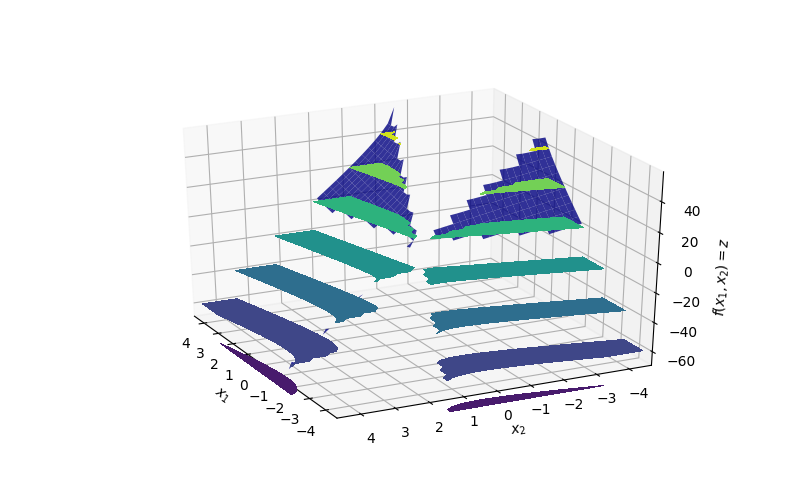
\includegraphics[width=\textwidth]{2_contorno.png}}
%   \caption{Curvas de nível e superfície da função, assim como o vetor de descida máxima}
%\end{figure}
